\documentclass[10pt,twocolumn,letterpaper]{article}
\usepackage[pagenumbers]{cvpr}
\usepackage{xeCJK}
\setmainfont{Times New Roman}
\setCJKmainfont[BoldFont=FandolSong-Bold,ItalicFont=FandolKai-Regular]{FandolSong-Regular}
\setCJKsansfont{FandolHei-Regular}
\usepackage{tabularx,array}
\usepackage{balance}
\definecolor{cvprblue}{rgb}{0.21,0.49,0.74}
\usepackage[breaklinks,colorlinks,allcolors=cvprblue]{hyperref}
\setlength{\emergencystretch}{1em}
\renewcommand{\abstractname}{摘要}
\renewcommand{\figurename}{图}
\renewcommand{\tablename}{表}
\renewcommand{\refname}{参考文献}
\hfuzz=0.2pt
\author{中文工作稿}
\date{}


\title{联邦长尾学习中的尾部类别知识保持与跨客户端知识迁移}

\begin{document}

\maketitle

\begin{abstract}

联邦长尾学习中，稀缺类别样本可能共同集中于少数客户端，使全局模型已经获得的尾部类别能力在后续训练中逐渐回落。本文在固定全局长尾样本池的条件下研究这一现象，并提出来源感知的协同适配框架。我们以客户端更新对类别预测间隔的正向作用衡量有效支持的集中程度，结合当前改善方向与历史预测间隔，对常规更新施加知识保持约束；进一步利用本地分类反馈学习客户端更新的低维矩阵组合，为全局模型补充学习支持。在 CIFAR-100-LT 的 Client-LT 实验中，完整配置的尾部类别准确率达到 72.63\%，整体准确率为 70.47\%。配对模块实验与同起点继续训练分析表明，来源感知权重和历史目标能够减少已有正确预测的丢失，更新组合则在此基础上提供补充收益。


\end{abstract}

\section*{1. 引言}

联邦学习通过客户端的本地训练与模型聚合学习共同的全局模型 [1]。在长尾视觉分类中，尾部类别的学习条件既取决于样本有多少，也取决于样本分布在哪里。若多种稀缺类别共同集中于少数客户端，这些客户端需要用有限样本支撑全局模型对相应类别的识别。随着其他客户端持续参与训练，这种识别能力能否保持，成为联邦长尾学习中的一个具体问题。


视觉语言模型提供了可迁移的视觉表示 [2]。LIFT 表明，这一起点能够支持长尾学习，但重度微调也可能损伤尾部类别性能 [3]。在联邦场景中，CAPT 通过类别感知提示改善适配 [4]，FedPuReL 则利用零样本预测指导知识保持 [5]。本文关注适配过程中进一步形成的能力：当模型已经从稀缺样本中获得改善，后续更新如何继续利用这一成果？


我们通过 Client-LT 划分考察这一问题：保持全局长尾样本池不变，将大部分尾部类别样本分配给同一组少数客户端。实验发现，全局模型能够先学会部分尾部类别样本，却在继续训练时重新分错；即使固定每类样本数和每个客户端的样本总量，改变类别样本的归属仍会改变保持表现（图 1）。因此，尾部类别学习需要同时考虑当前改善与已有能力的延续。


关键在于，样本所在位置不能完整描述类别的学习支持。客户端更新分析显示，不含目标类别样本的客户端也可能改善该类别的预测。由此，我们以更新对预测的实际作用连接知识保持与跨客户端知识迁移：对于正向作用集中于少数来源的类别功能，优先维护其已经达到的预测间隔；对于来自其他客户端的可用更新，通过目标类别反馈学习其组合方式。


基于这一思路，我们提出来源感知的协同适配框架。方法 A 在常规适配之后修正模型，根据当前客户端更新确定保持权重，并以历史预测间隔延续已经取得的改善。方法 B 复用本地训练产生的更新，学习各来源、各适配层的低维组合矩阵，将补充更新合并到同一个全局模型。二者分别作用于已有能力的保持和客户端知识的进一步利用。


本文的贡献包括：(1)通过相同样本池与固定边际对照，刻画客户端分布下的尾部类别保持问题；(2)提出来源感知的知识保持方法，将当前更新响应与历史预测间隔共同用于适配修正；(3)构建反馈驱动的客户端更新组合，并通过模块实验和样本预测变化分析检验保持与迁移的作用。


\begin{figure*}[t]\centering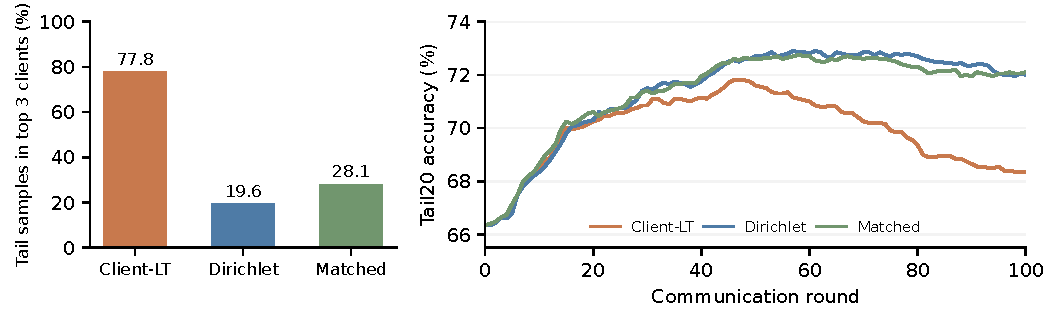
\includegraphics[width=\textwidth]{motivation.pdf}\caption{相同长尾样本池下的尾部类别保持。左：尾部样本最多的 3 个客户端所持尾部样本比例。右：相同交替因子训练策略下的 Tail20 准确率；Matched 同时固定类别总量与客户端样本总量。曲线均使用 rank-4 LoRA、全局 LA、样本量聚合与训练种子 42。}\end{figure*}

\section*{2. 相关工作}

\textbf{联邦长尾学习。} Logit adjustment 根据类别频率修正分类目标 [9]；FedLF、FedYoYo 和 FedReLa 分别从特征优化、自蒸馏和重标记等角度处理联邦类别不平衡 [10–12]。在基础模型适配中，CAPT 引入类别感知提示 [4]，FedPuReL 结合零样本知识保持与个性化残差学习 [5]。本文研究固定类别集合下的单一全局模型，以训练中持续取得的预测间隔作为动态保持目标。


\textbf{长尾视觉适配。} 长尾学习也受表示学习方式影响。DeiT-LT 通过蒸馏改善长尾数据上的视觉 Transformer 训练 [21]，类别外推方法利用相关辅助类别增强表示 [22]。对于视觉语言模型，预训练概念频率与类别性能之间的联系 [20]，以及重度微调对尾部类别的影响 [3]，共同说明适配需要关注具体类别的行为。本文使用本地类别反馈指导模型更新，并将训练过程中获得的改善纳入后续优化。


\textbf{知识保持与联邦低秩适配。} MOON 利用模型表示间的对比约束本地训练 [18]，FedNTD 通过非真类蒸馏维护全局知识 [6]，FedFTG 利用无数据蒸馏改进聚合后的全局模型 [19]。我们将保持对象具体化为类别预测间隔，并依据正向支持的集中程度分配保持权重。在参数层面，LoRA 提供低秩适配形式 [14]；FFA-LoRA、RoLoRA、FedSVD 和 LoRA-A$^2$ 分别研究因子冻结、交替优化、重参数化及自适应秩等设计 [7, 8, 15, 16]。本文在因子适配结果上施加功能约束，并利用低秩维度学习客户端更新的共享组合。


\section*{3. 问题与观察}

\textbf{客户端分布。} 设 $K$ 个客户端共同学习 $C$ 类全局分类模型，$n_{kc}$ 为客户端 $k$ 的类别 $c$ 样本数。类别总量 $n_c=\sum_k n_{kc}$ 描述全局长尾分布，$p(k\mid c)=n_{kc}/n_c$ 描述样本归属。Client-LT 通过集中程度 $\lambda_T$ 将尾部类别样本共同分配给占比为 $q_T$ 的客户端组，组内和组外分别采用 Dirichlet 分配。该组接收的期望尾部样本比例为 $q_T+(1-q_T)\lambda_T$。


在由 CIFAR-100 [17] 构建的固定长尾样本池中，尾部 20 类共有 153 张训练图像。取 $q_T=0.1$、$\lambda_T=0.75$ 时，30 个客户端中的 3 个持有 119 张尾部图像，占 77.78\%，但其全部样本仅占全局的 1.20\%。常规逐类 Dirichlet 划分中，尾部样本最多的 3 个客户端仅持有 19.61\%。


\textbf{已经获得的能力会回落。} 采用相同的 LoRA 交替训练策略，Client-LT 的 Tail20 准确率从峰值 71.80\% 回落至 68.35\%，常规 Dirichlet 从 72.90\% 回落至 72.00\%。进一步固定 $n_c$ 和 $n_k=\sum_c n_{kc}$，Matched 对照的回落为 0.65 个百分点。相同类别数量和客户端容量下仍存在的差异，使我们将保持对象落实到各客户端上的类别预测，而由当前更新响应识别其有效支持。


\textbf{有效支持超出标签所在位置。} 在 rank-2 的更新路径诊断中，我们将尾部类别预测分数的变化按来源及正负方向分解。Client-LT 下，不含目标类别样本客户端的累计正向作用为 17.642，含目标类别样本客户端为 6.874；前者同时具有负向作用。该结果说明，更新能否帮助目标类别需要由其预测作用判断，也为按反馈重新利用客户端更新提供了动机。诊断分数、积分过程与完整结果见补充材料 S2。


\section*{4. 来源感知的协同适配}

\begin{figure*}[t]\centering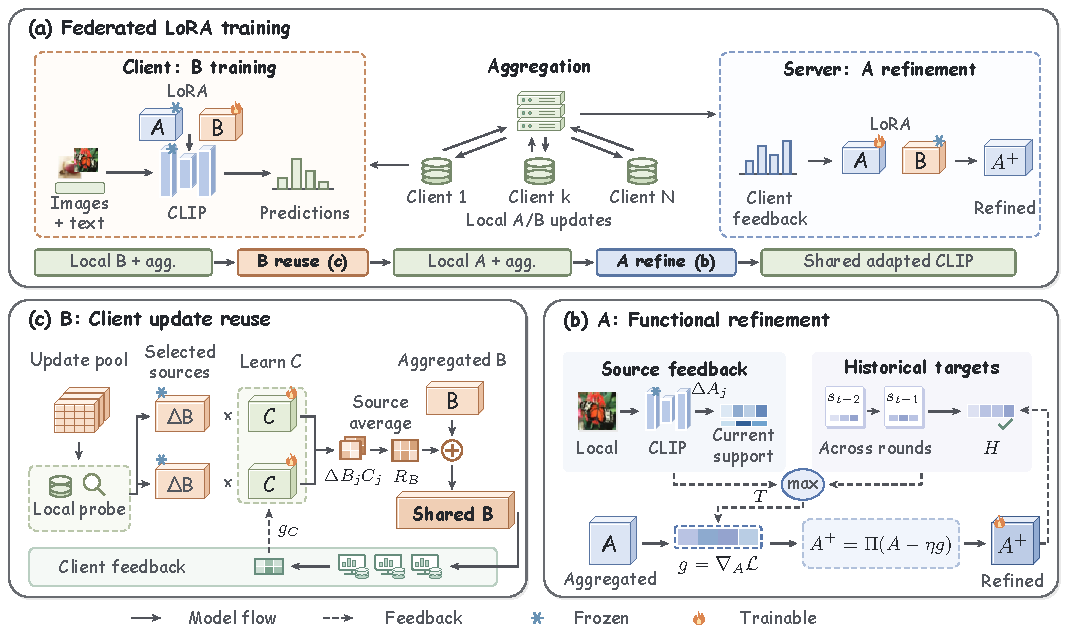
\includegraphics[width=\textwidth]{framework.pdf}\caption{整体框架。客户端更新首先形成普通聚合模型。方法 B 通过本地反馈学习更新组合；方法 A 利用来源响应和历史预测间隔修正适配结果。所有反馈图像保留在所属客户端，服务器根据反馈量与梯度协调优化。}\end{figure*}

\subsection*{4.1 整体框架}

我们在冻结的 CLIP 主干上加入 LoRA [14]，第 $\ell$ 层权重为 $W_\ell=W_{0\ell}+\gamma_\ell B_\ell A_\ell$。每轮先固定 $A_\ell$ 训练 $B_\ell$，再固定共同的 $B_\ell$ 训练 $A_\ell$。图 2 展示两个组件：方法 B 在普通 $B_\ell$ 聚合后形成补充更新；方法 A 在普通 $A_\ell$ 聚合后执行知识保持修正。下文用 $A$、$B$ 表示各层同名因子的集合，用 $\bar A$、$\bar B$ 表示普通聚合结果。


\subsection*{4.2 方法 A：来源感知的知识保持}

\textbf{用预测间隔描述类别能力。} 对每个非空客户端—类别组合 $q=(k,c)$，固定选取至多 8 张本地训练图像作为反馈集 $\mathcal W_q$。以原图和水平翻转两个视图 $v$，计算正确类别相对最强竞争类别的平均余弦分数差：


\begin{equation}\begin{aligned}F_{qv}(A)&=\frac{1}{|\mathcal W_q|}\sum_{x\in\mathcal W_q}
\!\Bigl[s_c(v(x);A)\\ &\quad-\max_{c'\ne c}s_{c'}(v(x);A)\Bigr].\end{aligned}\end{equation}

此时各客户端共享固定的因子 $B$。预测间隔越大，正确类别相对竞争类别的优势越强；方法 A 以这一优势的延续作为保持目标。


\textbf{根据有效支持分配保持权重。} 令 $A_t$ 为本阶段共同起点，$\Delta A_j$ 为客户端 $j$ 的本地更新。其对组合 $q$ 的一阶响应及有效来源数为


\begin{equation}\begin{aligned}
a_{qj}&=\left[\min_v\langle\nabla_A F_{qv}(A_t),\Delta A_j\rangle\right]_+,\\
N_q^{\mathrm{eff}}&=\frac{(\sum_j a_{qj})^2}{\sum_j a_{qj}^2},\qquad
\omega_q\propto\frac{1}{N_q^{\mathrm{eff}}}.
\end{aligned}\end{equation}

实现中仅保留大于 $10^{-6}$ 的正响应，并将有效组合的 $\omega_q$ 归一化。若正向作用集中于少数客户端，$N_q^{\mathrm{eff}}$ 较小，保持权重较高；若有更多来源提供相近强度的支持，权重相应降低。当前没有正响应时沿用此前的集中程度，初值为 $1/K$。


\textbf{让当前改善成为可延续的目标。} 对有正响应的组合，记正响应均值为 $u_q$，以 $F_{qv}(A_t)+0.5u_q$ 构造当前目标，并截断至预测间隔上界 2。历史目标 $H_q$ 则记录此前持续达到的间隔：每五轮取最终全局模型在两种视图上的最低值，当其超过已有记录至少 0.001 时更新。首次登记以初始模型间隔为改善参照。当前与历史目标共同给出


\begin{equation}T_{qv}=\max\left\{\min\bigl(2,F_{qv}(A_t)+0.5u_q\bigr),H_q\right\}.\end{equation}

仅有一种目标时使用该目标，两者均无效时不参与保持。当前目标利用本轮更新中的改善方向，历史目标使此前稳定获得的改善在后续回落时仍产生约束。


\textbf{在普通更新附近执行修正。} 以客户端更新的均方根幅度 $R=(K^{-1}\sum_j\|\Delta A_j\|^2)^{1/2}$ 确定修正尺度，令 $A(z)=\bar A+Rz$、$\|z\|\leq1$。保持损失只惩罚未达到目标的间隔：


\begin{equation}\mathcal L_{\mathrm{keep}}(z)=\sum_q\frac{\omega_q}{4}\sum_{v=1}^{2}
\left[\frac{T_{qv}-F_{qv}(A(z))}{\sigma_{qv}}\right]_+^2.\end{equation}

其中，$\sigma_{qv}=\max(10^{-3},R\|\nabla_A F_{qv}(A_t)\|)$ 按局部敏感度归一化。为同时考虑分类学习，令 $\widehat L$ 为反馈集上的 LA 损失，按客户端样本占比和本地类别频率加权，对相对普通提案的损失增加施加惩罚：


\begin{equation}\mathcal R_{\mathrm{cls}}(z)=\frac12\left[
\frac{\widehat L(A(z))-\widehat L(\bar A)}{\xi}
\right]_+^2,\end{equation}

其中 $\xi=\max(10^{-3},R\|\nabla_A\widehat L(\bar A)\|)$。最终优化


\begin{equation}\min_{\|z\|\leq1}\ \frac12\|z\|^2+
\lambda_F\mathcal L_{\mathrm{keep}}(z)+\mu_{\mathrm{cls}}\mathcal R_{\mathrm{cls}}(z).\end{equation}

三项分别限制修正幅度、维护类别间隔并约束分类损失增加。我们固定本轮目标与权重，从普通提案出发执行三步投影梯度更新，将修正后的因子用于下一轮训练。


\begin{table*}[t]\centering\caption{CIFAR-100-LT、Client-LT 上的分类准确率（\%）。同一骨干下各方法采用其对应训练流程；数值为种子 42 的末 20 轮均值。}\small\setlength{\tabcolsep}{3pt}

\begin{tabular*}{\textwidth}{@{\extracolsep{\fill}}lrrrr@{}}\toprule 方法 & Overall & Head20 & Middle60 & Tail20 \\\midrule

FedAvg-LoRA & 64.53 & 85.63 & 66.96 & 36.15 \\

FedAvg-LoRA＋LA & 71.18 & 78.45 & 72.37 & 60.36 \\

CAPT [4] & 66.82 & 79.27 & 61.22 & 71.18 \\

FedPuReL-Global [5] & 65.76 & 70.55 & 64.19 & 65.70 \\

FedNTD [6] & 64.15 & 86.12 & 65.78 & 37.28 \\

FedLF [10] & 67.73 & 77.36 & 70.54 & 49.66 \\

FedYoYo [11] & 64.46 & 67.90 & 67.69 & 51.36 \\

FedReLa [12] & 65.62 & 83.29 & 67.96 & 40.93 \\

RoLoRA [8] & 63.22 & 85.67 & 64.67 & 36.41 \\

FedSVD [15] & 67.27 & 82.92 & 63.68 & 62.37 \\

LoRA-A$^2$ [16] & 65.10 & 85.70 & 67.29 & 37.93 \\

本文方法 & 70.47 & 74.00 & 68.57 & 72.63 \\

\bottomrule\end{tabular*}\end{table*}

\subsection*{4.3 方法 B：反馈驱动的客户端更新组合}

方法 A 维护已经获得的类别能力，方法 B 进一步利用当轮客户端更新提供学习支持。我们先在普通聚合模型上探测各来源更新：若加入 $0.1\Delta B_j$ 能降低接收客户端上某个尾部类别的 LA 损失，且来源客户端不含该类别样本，则将该来源纳入候选。对各接收客户端的候选集合取并集，得到 $\mathcal D$。


对于来源 $j$ 和适配层 $\ell$，引入 $r\times r$ 矩阵 $C_{j\ell}$，构成共享补充：


\begin{equation}B_\ell(C)=\bar B_\ell+\frac{1}{|\mathcal D|}
\sum_{j\in\mathcal D}\Delta B_{j\ell}C_{j\ell}.\end{equation}

组合矩阵调整已有更新在低秩维度上的作用。所有含尾部类别样本的客户端组成反馈集合 $\mathcal R$，共同优化同一组 $C$：


\begin{equation}\mathcal J_B(C)=\frac{1}{|\mathcal R|}\sum_{k\in\mathcal R}L_k(C)
+\frac{\lambda_C}{|\mathcal D|L}\sum_{j,\ell}\|C_{j\ell}\|_F^2.\end{equation}

其中，$L$ 为适配层数；同时含尾部与非尾部样本时，$L_k=0.35L_{k,T}+0.65L_{k,N}$，仅含尾部样本时使用 $L_{k,T}$。尾部反馈引导补充更新改善稀缺类别，非尾部反馈同时约束其他类别的分类表现。每次从 $C=0$ 开始优化两步，再将补充合并到全局因子 $B$。推理阶段沿用单个全局 LoRA 模型。


\section*{5. 实验}

\subsection*{5.1 实验设置}

我们在 CIFAR-100-LT 的 Client-LT 划分上开展实验。全局不平衡因子为 100，训练图像共 10,847 张；30 个客户端每轮全部参与，共训练 100 轮。取 $q_T=0.1$、$\lambda_T=0.75$、组内 Dirichlet 参数 $\alpha_T=0.5$，划分种子为 42。按训练样本数量排序，前 20 类、中间 60 类和后 20 类分别记为 Head20、Middle60 和 Tail20，测试集每类 100 张图像。


使用 CLIP ViT-B/16，在视觉编码器最后三个 block 的 q/v 投影中加入 rank-4 LoRA。本地训练采用全局频率的 LA [9]、SGD 和批大小 32，学习率为 0.001。每轮训练 $B$ 三个 epoch，前 90 轮进一步训练 $A$ 一个 epoch。方法 A 取 $\lambda_F=10$、$\mu_{\mathrm{cls}}=1$；方法 B 在第 30、40、……、100 轮执行，取 $\lambda_C=0.001$。完整配置采用 joint 固定聚合权重，服务器在训练前依据各客户端类别计数求解，并用于两个因子的普通聚合；其目标函数及训练细节见补充材料 S1。


分类结果报告第 81—100 轮最终全局模型准确率的均值。表 1 使用训练种子 42；表 2 的配对模块实验使用原样本量聚合协议及种子 42、3407。对比方法使用共享 CLIP 骨干的实验实现：CAPT 为固定聚合版本，FedPuReL 为全局阶段，FedSVD 为非 DP 版本；其余适配方式见补充材料 S3。


\subsection*{5.2 分类性能}

表 1 中，完整配置的 Tail20 达到 72.63\%，在已测配置中最高；Overall 为 70.47\%。相对 CAPT 的已测版本，Tail20 和 Overall 分别提高 1.46 和 3.65 个百分点。FedAvg-LoRA＋LA 的 Overall 为 71.18\%，但 Tail20 为 60.36\%。各类别组的结果显示，本文配置将更多分类收益分配给尾部类别。


\subsection*{5.3 来源响应与历史目标的作用}

表 2 固定普通因子训练日程与样本量聚合方式，分别改变保持权重、目标和补充更新。A-flat 使用均匀保持权重，保留当前及历史目标；A-current 使用来源感知权重，仅保留当前目标。


\par\medskip\noindent\begin{minipage}{\columnwidth}\centering\captionof{table}{样本量聚合协议下的配对模块实验（\%）。列分别对应训练种子 42 和 3407，均报告末 20 轮平均准确率。}\small\setlength{\tabcolsep}{3pt}

\begin{tabularx}{\columnwidth}{Xrrrr}\toprule & \multicolumn{2}{c}{种子 42} & \multicolumn{2}{c}{种子 3407} \\ \cmidrule(lr){2-3}\cmidrule(lr){4-5} 配置 & Overall & Tail20 & Overall & Tail20 \\\midrule

普通交替训练 & 70.91 & 68.66 & 70.93 & 69.08 \\

A-flat & 70.71 & 70.06 & 70.78 & 70.53 \\

A-current & 70.87 & 68.94 & 70.87 & 69.32 \\

方法 A & 70.63 & 70.94 & 70.48 & 71.09 \\

方法 A＋方法 B & 70.70 & 71.16 & 70.51 & 71.22 \\

方法 A＋直接校准 & 70.67 & 71.26 & 70.43 & 71.31 \\

\bottomrule\end{tabularx}\end{minipage}\par\medskip

来源感知权重和历史目标均改善了尾部类别保持。方法 A 相对 A-flat 的 Tail20 分别提高 0.88 和 0.56 个百分点，表明按有效支持的集中程度分配约束优于均匀分配。相对 A-current，方法 A 的 Tail20 分别提高 2.00 和 1.77 个百分点，峰值至末轮的回落从 3.35/2.60 缩小至 1.00/0.50 个百分点。历史目标在当前响应之外保留了跨轮参照，使已经获得的改善持续参与后续优化。


相对普通交替训练，方法 A 的 Tail20 分别提高 2.27 和 2.01 个百分点，Overall 分别降低 0.28 和 0.45 个百分点。由此，保持约束的主要收益体现为尾部类别能力的延续，同时伴随整体分类表现的取舍。


\balance

\subsection*{5.4 保持收益对应哪些样本变化}

我们参照样本遗忘分析 [13]，从方法 A 的第 60、80 轮同一检查点分别继续训练五轮，比较普通更新、幅度匹配更新与方法 A。幅度匹配保留普通更新方向，仅将更新幅度匹配到修正后的大小。


\par\medskip\noindent\begin{minipage}{\columnwidth}\centering\captionof{table}{同起点五轮训练后的 Tail20 样本变化，共 2,000 张测试图像。两个起点准确率分别为 71.55\% 和 71.25\%。}\small\setlength{\tabcolsep}{3pt}

\begin{tabularx}{\columnwidth}{Xrrrr}\toprule 起点 & 更新 & 正确$\rightarrow$错误 & 错误$\rightarrow$正确 & Tail20，\% \\\midrule

60 & 普通更新 & 8 & 3 & 71.30 \\

60 & 幅度匹配 & 5 & 3 & 71.45 \\

60 & 方法 A & 2 & 2 & 71.55 \\

80 & 普通更新 & 15 & 3 & 70.65 \\

80 & 幅度匹配 & 8 & 1 & 70.90 \\

80 & 方法 A & 6 & 1 & 71.00 \\

\bottomrule\end{tabularx}\end{minipage}\par\medskip

表 3 中，方法 A 相对普通更新将正确$\rightarrow$错误样本数从 8/15 降至 2/6，相对幅度匹配也进一步减少；新增正确样本数则从 3/3 变为 2/1。因此，这组准确率收益主要来自更少的已有正确预测丢失。保持约束既改变了遗忘，也影响继续学习，样本变化使这两种作用得以区分。


\subsection*{5.5 客户端更新的补充作用}

加入方法 B 后，表 2 中 Tail20 分别提高 0.22 和 0.13 个百分点，Overall 分别提高 0.06 和 0.03 个百分点。作为对照，直接校准在 $B$ 的全坐标残差上优化，使用相同反馈、分组损失和步数，并逐步匹配有效权重增量的范数。方法 B 的 Tail20 略低于直接校准，Overall 略高，二者呈现不同的类别性能分配。


完整配置的八次组合中，候选并集均包含全部 30 个客户端，实际学习的是全部来源更新的矩阵变换。六个适配层、rank-4 共对应 2,880 个组合参数，最终残差合并后不增加推理分支。训练期间的额外反馈与修正开销见补充材料 S3。


\section*{6. 结论}

本文研究尾部类别样本集中于少数客户端时，全局模型已有分类能力的保持。来源感知的知识保持将当前更新的正向支持与历史预测间隔连接起来，客户端更新组合进一步利用本地反馈形成共享补充。CIFAR-100-LT 上的结果表明，尾部类别学习可以同时从已有能力的延续和客户端更新的复用中获益；样本层面分析进一步揭示，保持与继续学习共同决定最终的分类表现。


\clearpage

\typeout{MAIN-PAGES-END; REFERENCES-START-PAGE=\thepage}

\begin{thebibliography}{22}

\bibitem{r1}Brendan McMahan, Eider Moore, Daniel Ramage, Seth Hampson, Blaise Agüera y Arcas. \href{https://proceedings.mlr.press/v54/mcmahan17a.html}{Communication-Efficient Learning of Deep Networks from Decentralized Data}. AISTATS, 2017.

\bibitem{r2}Alec Radford, Jong Wook Kim, Chris Hallacy, et al. \href{https://proceedings.mlr.press/v139/radford21a.html}{Learning Transferable Visual Models From Natural Language Supervision}. ICML, 2021.

\bibitem{r3}Jiang-Xin Shi, Tong Wei, Zhi Zhou, Jie-Jing Shao, Xin-Yan Han, Yu-Feng Li. \href{https://proceedings.mlr.press/v235/shi24g.html}{Long-Tail Learning with Foundation Model: Heavy Fine-Tuning Hurts}. ICML, 2024.

\bibitem{r4}Shihao Hou, Xinyi Shang, Shreyank N Gowda, et al. \href{https://arxiv.org/abs/2503.06993}{CAPT: Class-Aware Prompt Tuning for Federated Long-Tailed Learning with Vision-Language Model}. arXiv:2503.06993, 2025.

\bibitem{r5}Shihao Hou, Chikai Shang, Zhiheng Yang, et al. \href{https://openaccess.thecvf.com/content/CVPR2026/html/Hou_Fine-Tuning_Impairs_the_Balancedness_of_Foundation_Models_in_Long-tailed_Personalized_CVPR_2026_paper.html}{Fine-Tuning Impairs the Balancedness of Foundation Models in Long-tailed Personalized Federated Learning}. CVPR, 2026.

\bibitem{r6}Gihun Lee, Minchan Jeong, Yongjin Shin, Sangmin Bae, Se-Young Yun. \href{https://proceedings.neurips.cc/paper_files/paper/2022/hash/fadec8f2e65f181d777507d1df69b92f-Abstract-Conference.html}{Preservation of the Global Knowledge by Not-True Distillation in Federated Learning}. NeurIPS, 2022.

\bibitem{r7}Youbang Sun, Zitao Li, Yaliang Li, Bolin Ding. \href{https://proceedings.iclr.cc/paper_files/paper/2024/hash/4e243e95c913b367775d71d7182b99d9-Abstract-Conference.html}{Improving LoRA in Privacy-preserving Federated Learning}. ICLR, 2024.

\bibitem{r8}Shuangyi Chen, Yuanxin Guo, Yue Ju, Hardik Dalal, Zhongwen Zhu, Ashish Khisti. \href{https://proceedings.neurips.cc/paper_files/paper/2025/hash/adf17e7346b6be4c2f2bb40de572e5bc-Abstract-Conference.html}{Robust Federated Finetuning of LLMs via Alternating Optimization of LoRA}. NeurIPS, 2025.

\bibitem{r9}Aditya Krishna Menon, Sadeep Jayasumana, Ankit Singh Rawat, Himanshu Jain, Andreas Veit, Sanjiv Kumar. \href{https://openreview.net/pdf?id=37nvvqkCo5}{Long-tail learning via logit adjustment}. ICLR, 2021.

\bibitem{r10}Xiuhua Lu, Peng Li, Xuefeng Jiang. \href{https://proceedings.mlr.press/v260/lu25a.html}{FedLF: Adaptive Logit Adjustment and Feature Optimization in Federated Long-Tailed Learning}. Proceedings of the 16th Asian Conference on Machine Learning, PMLR 260, 2025.

\bibitem{r11}Shanshan Yan, Zexi Li, Chao Wu, et al. \href{https://openaccess.thecvf.com/content/ICCV2025/html/Yan_You_Are_Your_Own_Best_Teacher_Achieving_Centralized-level_Performance_in_ICCV_2025_paper.html}{You Are Your Own Best Teacher: Achieving Centralized-level Performance in Federated Learning under Heterogeneous and Long-tailed Data}. ICCV, 2025.

\bibitem{r12}Guangzheng Hu, Patricia Menendez, Feng Liu, Mingming Gong, Guanghui Wang, Liuhua Peng. \href{https://proceedings.mlr.press/v306/hu26ao.html}{FedReLa: Imbalanced Federated Learning via Re-Labeling}. ICML, 2026.

\bibitem{r13}Mariya Toneva, Alessandro Sordoni, Remi Tachet des Combes, Adam Trischler, Yoshua Bengio, Geoffrey J. Gordon. \href{https://arxiv.org/abs/1812.05159}{An Empirical Study of Example Forgetting during Deep Neural Network Learning}. ICLR, 2019.

\bibitem{r14}Edward J. Hu, Yelong Shen, Phillip Wallis, et al. \href{https://arxiv.org/abs/2106.09685}{LoRA: Low-Rank Adaptation of Large Language Models}. arXiv:2106.09685, 2021.

\bibitem{r15}Seanie Lee, Sangwoo Park, Dong Bok Lee, et al. \href{https://arxiv.org/abs/2505.12805}{FedSVD: Adaptive Orthogonalization for Private Federated Learning with LoRA}. NeurIPS, 2025.

\bibitem{r16}Jabin Koo, Minwoo Jang, Jungseul Ok. \href{https://aclanthology.org/2025.acl-long.19/}{Towards Robust and Efficient Federated Low-Rank Adaptation with Heterogeneous Clients}. ACL, 2025.

\bibitem{r17}Alex Krizhevsky. \href{https://www.cs.toronto.edu/~kriz/learning-features-2009-TR.pdf}{Learning Multiple Layers of Features from Tiny Images}. University of Toronto, Technical Report, 2009.

\bibitem{r18}Qinbin Li, Bingsheng He, Dawn Song. \href{https://openaccess.thecvf.com/content/CVPR2021/html/Li_Model-Contrastive_Federated_Learning_CVPR_2021_paper.html}{Model-Contrastive Federated Learning}. CVPR, 2021.

\bibitem{r19}Lin Zhang, Li Shen, Liang Ding, Dacheng Tao, Ling-Yu Duan. \href{https://openaccess.thecvf.com/content/CVPR2022/html/Zhang_Fine-Tuning_Global_Model_via_Data-Free_Knowledge_Distillation_for_Non-IID_Federated_CVPR_2022_paper.html}{Fine-Tuning Global Model via Data-Free Knowledge Distillation for Non-IID Federated Learning}. CVPR, 2022.

\bibitem{r20}Shubham Parashar, Zhiqiu Lin, Tian Liu, Xiangjue Dong, Yanan Li, Deva Ramanan, James Caverlee, Shu Kong. \href{https://openaccess.thecvf.com/content/CVPR2024/html/Parashar_The_Neglected_Tails_in_Vision-Language_Models_CVPR_2024_paper.html}{The Neglected Tails in Vision-Language Models}. CVPR, 2024.

\bibitem{r21}Harsh Rangwani, Pradipto Mondal, Mayank Mishra, Ashish Ramayee Asokan, R. Venkatesh Babu. \href{https://openaccess.thecvf.com/content/CVPR2024/html/Rangwani_DeiT-LT_Distillation_Strikes_Back_for_Vision_Transformer_Training_on_Long-Tailed_CVPR_2024_paper.html}{DeiT-LT: Distillation Strikes Back for Vision Transformer Training on Long-Tailed Datasets}. CVPR, 2024.

\bibitem{r22}Shizhen Zhao, Xin Wen, Jiahui Liu, Chuofan Ma, Chunfeng Yuan, Xiaojuan Qi. \href{https://openaccess.thecvf.com/content/CVPR2025/html/Zhao_Learning_from_Neighbors_Category_Extrapolation_for_Long-Tail_Learning_CVPR_2025_paper.html}{Learning from Neighbors: Category Extrapolation for Long-Tail Learning}. CVPR, 2025.

\end{thebibliography}

\end{document}